% ============================================================
%  CHAPTER 1: MEASUREMENT AND UNITS
%  The Physics Codex: A Complete University Foundation
%  Korede Samuel Omotosho (Falcon)
%  Aurikrex Learning Systems, 2026
%
%  File: chapters/part1/ch01_measurement.tex
% ============================================================

\chapter{Measurement and Units}
\label{ch:measurement}

% ============================================================
\chapterquote{Measure what is measurable, and make measurable
what is not so.}{Galileo Galilei}

% ============================================================
\begin{objectivebox}
By the end of this chapter, you should be able to:
\begin{enumerate}[noitemsep]
  \item Explain why measurement and units are fundamental
  to Physics
  \item State and apply the seven SI fundamental quantities and
  their units
  \item Use metric prefixes to express very large and very
  small quantities
  \item Express measurements in standard form (scientific
  notation)
  \item Define and distinguish between scalar and vector
  quantities
  \item Determine the dimensions of physical quantities
  and use dimensional analysis to check equations
  \item Define significant figures and apply the rules for
  rounding and arithmetic with significant figures
  \item Estimate physical quantities using order-of-magnitude
  reasoning
\end{enumerate}
\end{objectivebox}

\vspace{0.4cm}

\minitoc

\vspace{0.5cm}

% ============================================================
\section{Why Measurement Matters}
\label{sec:why_measurement}
% ============================================================

Before any Physics can be done, something must be measured.
This seems obvious, yet its implications are profound. When
Galileo rolled balls down inclined planes in the 1590s, he
was not merely observing --- he was \textit{measuring}. He
timed the balls using his own pulse, then later using a
water clock, counting the flow of water to establish
precisely how far a ball travelled in a given time. That act
of careful measurement, repeated and refined, gave us the
first quantitative laws of motion.

Physics is, at its core, the science of measurement. Every
law, every equation, every theory in this textbook rests on
measurements that were made carefully, recorded honestly, and
repeated until the results were trustworthy. Understanding
how measurement works --- what units mean, how to handle
uncertainty, how to express results correctly --- is not
preliminary to Physics. It \textit{is} Physics.

\begin{historybox}[The Metre's Origin]
Before the 19th century, every country used its own units.
An English foot was different from a French foot. Trade was
difficult; scientific communication was a mess. In 1791,
following the French Revolution, French scientists proposed
a universal system based on nature itself. The metre was
defined as one ten-millionth of the distance from the
Earth's equator to the North Pole along a meridian passing
through Paris. In 1960 this became the International System
of Units (SI), now used by every scientist on Earth and by
every country except three --- the United States, Liberia,
and Myanmar --- for official trade and industry.
\end{historybox}

% ============================================================
\section{Physical Quantities}
\label{sec:physical_quantities}
% ============================================================

A \textbf{physical quantity} is anything that can be measured.
Mass, length, time, temperature, electric current, speed,
force --- these are all physical quantities. Every physical
quantity consists of two parts: a \textbf{numerical value}
and a \textbf{unit}.

Writing ``the length is 5'' is meaningless. Five what? Five
metres? Five kilometres? Five centimetres? The unit is not
optional --- it is half the answer. A student who writes
$v = 30$ when calculating speed has given an incomplete and
potentially dangerous answer. The correct answer is
$v = 30\ \text{m\,s}^{-1}$.

\begin{keybox}[Physical Quantity = Number + Unit]
Every measurement must include both a numerical value and
a unit. A number without a unit is not a measurement --- it
is merely a number.
\[
  \text{Physical Quantity} = \text{Numerical Value}
  \times \text{Unit}
\]
Example: $m = 5.0\ \text{kg}$, $\ell = 3.2\ \text{m}$,
$t = 12.5\ \text{s}$
\end{keybox}

\subsection{Fundamental Quantities and Derived Quantities}

All physical quantities can be divided into two categories.

\begin{definitionbox}[Fundamental Quantity]
A \textbf{fundamental quantity} is a physical quantity that is
defined independently and cannot be expressed in terms of
other physical quantities. The SI system defines seven fundamental
quantities.
\end{definitionbox}

\begin{definitionbox}[Derived Quantity]
A \textbf{derived quantity} is a physical quantity that is
defined in terms of two or more fundamental quantities through a
mathematical relationship.
\end{definitionbox}

Table~\ref{tab:si_base} shows the seven SI fundamental quantities,
their symbols, and their units.

\begin{table}[H]
\centering
\caption{The Seven SI Fundamental Quantities}
\label{tab:si_base}
\begin{tabular}{llll}
\toprule
\textbf{Fundamental Quantity} & \textbf{Symbol} &
\textbf{SI Unit} & \textbf{Unit Symbol}\\
\midrule
Length          & $\ell$ or $L$ & metre      & m\\
Mass            & $m$           & kilogram   & kg\\
Time            & $t$           & second     & s\\
Electric current& $I$           & ampere     & A\\
Temperature     & $T$           & kelvin     & K\\
Amount of substance & $n$       & mole       & mol\\
Luminous intensity & $I_v$      & candela    & cd\\
\bottomrule
\end{tabular}
\end{table}

\begin{realworldbox}[Why These Seven?]
These seven were not chosen arbitrarily. They were chosen
because they are \textit{independent} of each other --- you
cannot derive any one of them from the other six. Everything
else in Physics --- speed, force, energy, electric charge,
pressure --- can be built from combinations of these seven.
Think of them as the seven primary colours from which every
other colour in Physics is mixed.
\end{realworldbox}

Examples of derived quantities built from fundamental quantities:

\begin{align*}
  \text{Speed} &= \frac{\text{length}}{\text{time}}
  = \frac{\text{m}}{\text{s}} = \text{m\,s}^{-1}\\[6pt]
  \text{Force} &= \text{mass} \times \text{acceleration}
  = \text{kg} \times \text{m\,s}^{-2}
  = \text{kg\,m\,s}^{-2} = \text{N}\\[6pt]
  \text{Energy} &= \text{force} \times \text{distance}
  = \text{N\,m} = \text{kg\,m}^2\text{s}^{-2} = \text{J}
\end{align*}

% ============================================================
\section{The SI System and Metric Prefixes}
\label{sec:si_prefixes}
% ============================================================

The SI system is a \textbf{decimal system} --- every unit
is related to every other by powers of ten. This makes
calculations vastly simpler than systems like the imperial
system where 12 inches make a foot, 3 feet make a yard, and
1760 yards make a mile.

When quantities are very large or very small, we use
\textbf{prefixes} to avoid writing long strings of zeros.
Table~\ref{tab:prefixes} lists the most important prefixes.

\begin{table}[H]
\centering
\caption{SI Metric Prefixes}
\label{tab:prefixes}
\begin{tabular}{lllll}
\toprule
\textbf{Prefix} & \textbf{Symbol} & \textbf{Factor} &
\textbf{Example} & \textbf{Meaning}\\
\midrule
tera  & T & $10^{12}$ & 1 Tm & $10^{12}$ metres\\
giga  & G & $10^9$    & 1 GW & $10^9$ watts\\
mega  & M & $10^6$    & 1 MHz& $10^6$ hertz\\
kilo  & k & $10^3$    & 1 km & $10^3$ metres\\
hecto & h & $10^2$    & 1 hPa& $10^2$ pascals\\
deca  & da& $10^1$    & 1 dag& $10$ grams\\
---   & ---& $10^0 = 1$& ---  & base unit\\
deci  & d & $10^{-1}$ & 1 dm & $0.1$ metres\\
centi & c & $10^{-2}$ & 1 cm & $0.01$ metres\\
milli & m & $10^{-3}$ & 1 mm & $0.001$ metres\\
micro & $\mu$ & $10^{-6}$ & 1 $\mu$m & $10^{-6}$ metres\\
nano  & n & $10^{-9}$ & 1 nm & $10^{-9}$ metres\\
pico  & p & $10^{-12}$& 1 pm & $10^{-12}$ metres\\
femto & f & $10^{-15}$& 1 fm & $10^{-15}$ metres\\
\bottomrule
\end{tabular}
\end{table}

\begin{realworldbox}[Prefixes in Everyday Nigerian Life]
You encounter SI prefixes constantly without realising it.
When your phone shows your data usage as 2.4 GB, that is
$2.4 \times 10^9$ bytes. When a generator is rated at
3.5 kVA, that is $3.5 \times 10^3$ volt-amperes. When a
nurse takes your blood pressure and says your pulse is
72 bpm (beats per minute), the frequency of your heartbeat
is approximately 1.2 Hz. When a civil engineer says a road
is 14 km long, that is $14{,}000$ metres. The prefix system
is everywhere.
\end{realworldbox}

\subsection{Converting Between Units}

Converting from one unit to another requires multiplying by
a \textbf{conversion factor} --- a fraction equal to 1 whose
numerator and denominator represent the same quantity in
different units.

\begin{examplebox}[1.1]
\stepcounter{workedexample}
Convert $8.5\ \text{km}$ to metres.
\end{examplebox}

\begin{solutionbox}
Since $1\ \text{km} = 10^3\ \text{m} = 1000\ \text{m}$:
\[
  8.5\ \text{km}
  = 8.5 \times 10^3\ \text{m}
  = 8500\ \text{m}
\]
\end{solutionbox}

\begin{examplebox}[1.2]
\stepcounter{workedexample}
Convert a speed of $90\ \text{km\,h}^{-1}$ to
$\text{m\,s}^{-1}$.
\end{examplebox}

\begin{solutionbox}
We need to convert kilometres to metres AND hours to seconds:
\begin{align*}
  90\ \frac{\text{km}}{\text{h}}
  &= 90 \times \frac{1000\ \text{m}}{3600\ \text{s}}\\[6pt]
  &= 90 \times \frac{1000}{3600}\ \text{m\,s}^{-1}\\[6pt]
  &= 90 \times \frac{5}{18}\ \text{m\,s}^{-1}\\[6pt]
  &= 25\ \text{m\,s}^{-1}
\end{align*}

\textbf{Shortcut:} To convert km\,h$^{-1}$ to m\,s$^{-1}$,
divide by 3.6. To convert m\,s$^{-1}$ to km\,h$^{-1}$,
multiply by 3.6.
\end{solutionbox}

\begin{examtipbox}
The conversion $\div 3.6$ (km\,h$^{-1}$ to m\,s$^{-1}$) and
$\times 3.6$ (m\,s$^{-1}$ to km\,h$^{-1}$) appears in
almost every kinematics problem in UTME. Memorise it.
\end{examtipbox}

\begin{examplebox}[1.3]
\stepcounter{workedexample}
The density of iron is $7.87\ \text{g\,cm}^{-3}$.
Express this in $\text{kg\,m}^{-3}$.
\end{examplebox}

\begin{solutionbox}
We need to convert grams to kilograms ($\div 1000$) and
cubic centimetres to cubic metres.

Since $1\ \text{cm} = 10^{-2}\ \text{m}$:
\[
  1\ \text{cm}^3 = (10^{-2})^3\ \text{m}^3
  = 10^{-6}\ \text{m}^3
\]
Therefore:
\begin{align*}
  7.87\ \frac{\text{g}}{\text{cm}^3}
  &= 7.87 \times \frac{10^{-3}\ \text{kg}}{10^{-6}\ \text{m}^3}\\[6pt]
  &= 7.87 \times 10^{3}\ \text{kg\,m}^{-3}\\[6pt]
  &= 7870\ \text{kg\,m}^{-3}
\end{align*}

\textbf{Note:} To convert g\,cm$^{-3}$ to kg\,m$^{-3}$,
multiply by 1000.
\end{solutionbox}

% ============================================================
\section{Standard Form (Scientific Notation)}
\label{sec:standard_form}
% ============================================================

\begin{definitionbox}[Standard Form]
A number written in \textbf{standard form} (also called
\textbf{scientific notation}) is expressed as:
\[
  A \times 10^n
\]
where $1 \leq A < 10$ and $n$ is an integer (positive,
negative, or zero).
\end{definitionbox}

Standard form is essential in Physics because the quantities
we work with range enormously. The mass of an electron is
$0.000\,000\,000\,000\,000\,000\,000\,000\,000\,000\,911$
kilograms. The distance from Earth to the nearest star
(Proxima Centauri) is roughly
$40\,000\,000\,000\,000\,000$ metres. Expressing these
numbers without standard form is both impractical and prone
to error.

\begin{align*}
  m_e &= 9.11 \times 10^{-31}\ \text{kg}\\
  d_{Proxima} &\approx 4.0 \times 10^{16}\ \text{m}
\end{align*}

\begin{examplebox}[1.4]
\stepcounter{workedexample}
Express the following in standard form:\\
(a)\ $0.000\,047\ \text{m}$\qquad
(b)\ $93\,000\,000\ \text{km}$\qquad
(c)\ $0.0000000000000000001602\ \text{C}$
\end{examplebox}

\begin{solutionbox}
\textbf{(a)} Move the decimal point 5 places to the right:
\[
  0.000\,047\ \text{m} = 4.7 \times 10^{-5}\ \text{m}
\]

\textbf{(b)} Move the decimal point 7 places to the left:
\[
  93\,000\,000\ \text{km} = 9.3 \times 10^7\ \text{km}
\]

\textbf{(c)} This is the elementary charge. Move the
decimal 19 places to the right:
\[
  1.602 \times 10^{-19}\ \text{C}
\]
\end{solutionbox}

% ============================================================
\section{Dimensional Analysis}
\label{sec:dimensional_analysis}
% ============================================================

\begin{definitionbox}[Dimension]
The \textbf{dimension} of a physical quantity describes what
type of quantity it is --- in terms of the fundamental quantities.
We use square brackets to denote dimensions. The fundamental
dimensions are:
\[
\begin{aligned}
  \relax[M] &= \text{mass}, & [L] &= \text{length}, & [T] &= \text{time},\\
  [I] &= \text{electric current}, & [\Theta] &= \text{temperature}
\end{aligned}
\]
\end{definitionbox}

Dimensions are not the same as units. Metres, feet,
centimetres, and miles all have the dimension $[L]$ even
though they are different units. The dimension tells you
\textit{what kind} of quantity you have; the unit tells you
\textit{how much} of it you measured.

\subsection{Finding the Dimensions of Derived Quantities}

To find the dimension of a derived quantity, substitute the
dimensions of the fundamental quantities into its defining equation.

\vspace{0.3cm}

\textbf{Speed:}
\[
  v = \frac{\text{distance}}{\text{time}}
  \implies [v] = \frac{[L]}{[T]} = [L\,T^{-1}]
\]

\textbf{Force:}
\[
  F = ma
  \implies [F] = [M][L\,T^{-2}] = [M\,L\,T^{-2}]
\]

\textbf{Energy (Work):}
\[
  W = Fd
  \implies [W] = [M\,L\,T^{-2}][L] = [M\,L^2\,T^{-2}]
\]

\textbf{Pressure:}
\[
  P = \frac{F}{A}
  \implies [P] = \frac{[M\,L\,T^{-2}]}{[L^2]}
  = [M\,L^{-1}\,T^{-2}]
\]

\subsection{The Principle of Homogeneity}

\begin{lawbox}[Principle of Dimensional Homogeneity]
In any valid physical equation, every term on both sides
of the equation must have the \textbf{same dimensions}.
You cannot add a length to a time. You cannot equate a
force to an energy. If the dimensions do not match, the
equation is wrong.
\end{lawbox}

This gives us a powerful tool for checking equations and
for deriving relationships between quantities --- a method
called \textbf{dimensional analysis}.

\begin{examplebox}[1.5]
\stepcounter{workedexample}
Check whether the equation $v^2 = u^2 + 2as$ is
dimensionally consistent, where $v$ and $u$ are speeds,
$a$ is acceleration, and $s$ is displacement.
\end{examplebox}

\begin{solutionbox}
Find the dimension of each term:
\begin{align*}
  [v^2] &= [L\,T^{-1}]^2 = [L^2\,T^{-2}]\\[4pt]
  [u^2] &= [L^2\,T^{-2}]\\[4pt]
  [2as] &= [L\,T^{-2}][L] = [L^2\,T^{-2}]
\end{align*}

All three terms have dimension $[L^2\,T^{-2}]$.
The equation is \textbf{dimensionally consistent}.

\textit{Note:} Dimensional consistency does not guarantee
the equation is correct --- the numerical factor 2 cannot
be verified by dimensional analysis. But dimensional
inconsistency guarantees the equation is wrong.
\end{solutionbox}

\begin{examplebox}[1.6]
\stepcounter{workedexample}
A student writes the following equation for the period $T$
of a simple pendulum of length $L$ swinging under gravity $g$:
\[
  T = 2\pi\sqrt{\frac{g}{L}}
\]
Use dimensional analysis to show this equation is incorrect.
\end{examplebox}

\begin{solutionbox}
The left side has dimension $[T]$ (time).

The right side: $2\pi$ is dimensionless. Now check
$\sqrt{g/L}$:
\[
  \left[\frac{g}{L}\right]
  = \frac{[L\,T^{-2}]}{[L]}
  = [T^{-2}]
\]
\[
  \left[\sqrt{\frac{g}{L}}\right] = [T^{-1}]
\]

The right side has dimension $[T^{-1}]$, which is NOT equal
to $[T]$.

\textbf{Conclusion:} The equation is dimensionally
inconsistent and therefore incorrect. The correct equation
is $T = 2\pi\sqrt{L/g}$.
\end{solutionbox}

\begin{examplebox}[1.7]
\stepcounter{workedexample}
The period $T$ of a planet orbiting the Sun depends on its
orbital radius $r$, the mass of the Sun $M_s$, and the
gravitational constant $G$ (dimensions
$[M^{-1}\,L^3\,T^{-2}]$). Use dimensional analysis to find
the relationship between these quantities.
\end{examplebox}

\begin{solutionbox}
Assume $T \propto r^a\, M_s^b\, G^c$.

Writing dimensions:
\[
  [T] = [L]^a\,[M]^b\,[M^{-1}\,L^3\,T^{-2}]^c
\]
\[
  [T^1] = [M^{b-c}\,L^{a+3c}\,T^{-2c}]
\]

Equating powers:
\begin{align*}
  T&:\quad 1 = -2c \implies c = -\tfrac{1}{2}\\
  M&:\quad 0 = b - c \implies b = c = -\tfrac{1}{2}\\
  L&:\quad 0 = a + 3c \implies a = -3c = \tfrac{3}{2}
\end{align*}

Therefore:
\[
  T \propto r^{3/2}\,M_s^{-1/2}\,G^{-1/2}
  = \sqrt{\frac{r^3}{G M_s}}
\]

This is Kepler's Third Law, derived purely from dimensions.
\end{solutionbox}

% ============================================================
\section{Significant Figures}
\label{sec:sig_figs}
% ============================================================

\begin{definitionbox}[Significant Figures]
The \textbf{significant figures} (s.f.) of a measurement
are the digits that carry meaningful information about its
precision. They include all certain digits plus the first
uncertain (estimated) digit.
\end{definitionbox}

\subsection{Rules for Counting Significant Figures}

\begin{enumerate}
  \item \textbf{All non-zero digits are significant.}\\
  $347$ has 3 s.f.\quad $5.82$ has 3 s.f.

  \item \textbf{Zeros between non-zero digits are
  significant.}\\
  $4007$ has 4 s.f.\quad $3.05$ has 3 s.f.

  \item \textbf{Leading zeros (zeros before the first
  non-zero digit) are NOT significant.}\\
  $0.0042$ has 2 s.f.\quad $0.507$ has 3 s.f.

  \item \textbf{Trailing zeros after the decimal point
  ARE significant.}\\
  $2.500$ has 4 s.f.\quad $0.0300$ has 3 s.f.

  \item \textbf{Trailing zeros in a whole number without
  a decimal point are ambiguous.}\\
  $3700$ could have 2, 3, or 4 s.f. Write in standard
  form to be clear: $3.7 \times 10^3$ (2 s.f.),
  $3.70 \times 10^3$ (3 s.f.), $3.700 \times 10^3$ (4 s.f.)
\end{enumerate}

\subsection{Arithmetic with Significant Figures}

\textbf{Multiplication and Division:} The result has the
same number of significant figures as the measurement with
the \textit{fewest} significant figures.

\[
  \frac{4.56 \times 1.4}{3.0}
  = \frac{6.384}{3.0} = 2.128 \approx 2.1
  \quad \text{(2 s.f., limited by 1.4 and 3.0)}
\]

\textbf{Addition and Subtraction:} The result has the same
number of \textit{decimal places} as the measurement with
the \textit{fewest} decimal places.

\[
  12.52 + 349.0 + 8.24 = 369.76 \approx 369.8
  \quad \text{(1 d.p., limited by 349.0)}
\]

\begin{misconceptionbox}
Many students confuse \textit{accuracy} and
\textit{precision}. These are not the same thing.
\textbf{Accuracy} refers to how close a measurement is
to the true value. \textbf{Precision} refers to how
reproducible (consistent) the measurements are. A
precise measurement that is not accurate is like a gun
that puts every bullet in the same wrong place. You want
both accuracy and precision.
\end{misconceptionbox}

% ============================================================
\section{Errors and Uncertainty}
\label{sec:errors}
% ============================================================

No measurement is perfect. Every measurement has an
associated \textbf{uncertainty} that reflects the
limitations of the measuring instrument and the experimenter.

\begin{definitionbox}[Types of Error]
\textbf{Systematic error} is a consistent, repeatable error
that shifts all measurements in the same direction (always
too high or always too low). Caused by instrument
miscalibration, incorrect technique, or environmental
factors. Cannot be reduced by repeating measurements.
Example: a ruler with its zero mark worn away so that every
measurement reads 1 mm too high.

\vspace{0.4cm}

\textbf{Random error} is unpredictable, equally likely to
be positive or negative. Caused by fluctuations in the
experiment, observer limitations, or environmental
variations. Can be reduced by taking many measurements and
averaging.
\end{definitionbox}

\begin{definitionbox}[Absolute and Relative Uncertainty]
The \textbf{absolute uncertainty} $\Delta x$ of a
measurement $x$ is the range within which the true value
almost certainly lies:
\[
  x = x_0 \pm \Delta x
\]
The \textbf{relative (fractional) uncertainty} is:
\[
  \text{Relative uncertainty} = \frac{\Delta x}{x_0}
\]
The \textbf{percentage uncertainty} is:
\[
  \text{Percentage uncertainty} = \frac{\Delta x}{x_0}
  \times 100\%
\]
\end{definitionbox}

\textbf{Propagation of uncertainties:}

For quantities combined by addition or subtraction,
\textit{add the absolute uncertainties}:
\[
  z = x + y \implies \Delta z = \Delta x + \Delta y
\]

For quantities combined by multiplication, division, or
powers, \textit{add the relative uncertainties}:
\[
  z = x^a\,y^b \implies
  \frac{\Delta z}{z} = |a|\frac{\Delta x}{x}
  + |b|\frac{\Delta y}{y}
\]

\begin{examplebox}[1.8]
\stepcounter{workedexample}
A rectangular metal plate is measured with a ruler. The
length is $L = 12.4 \pm 0.1\ \text{cm}$ and the width is
$W = 7.6 \pm 0.1\ \text{cm}$.

\smallskip

(a) Calculate the area with its absolute uncertainty.

(b) Calculate the percentage uncertainty in the area.
\end{examplebox}

\begin{solutionbox}
\textbf{(a)} Area:
\[
  A = LW = 12.4 \times 7.6 = 94.24\ \text{cm}^2
\]

For multiplication, add relative uncertainties:
\[
  \frac{\Delta A}{A} = \frac{\Delta L}{L}
  + \frac{\Delta W}{W}
  = \frac{0.1}{12.4} + \frac{0.1}{7.6}
  = 0.00806 + 0.01316 = 0.0212
\]
\[
  \Delta A = 0.0212 \times 94.24 \approx 2.0\ \text{cm}^2
\]
\[
  \boxed{A = 94 \pm 2\ \text{cm}^2}
\]

Note: We round to 2 significant figures in the uncertainty,
and the area is then given to the same decimal place as
the uncertainty.

\textbf{(b)} Percentage uncertainty:
\[
  \frac{\Delta A}{A} \times 100\%
  = 0.0212 \times 100\% = 2.1\%
\]
\end{solutionbox}

% ============================================================
\section{Order of Magnitude Estimation}
\label{sec:order_of_magnitude}
% ============================================================

\begin{definitionbox}[Order of Magnitude]
The \textbf{order of magnitude} of a quantity is the power
of ten closest to its value. Two quantities are said to
differ by an order of magnitude for every factor of ten
between them.
\end{definitionbox}

Order-of-magnitude estimation --- sometimes called a
\textbf{Fermi estimate} after the physicist Enrico Fermi,
who was famous for making rapid, accurate estimates from
first principles --- is one of the most useful skills a
physicist (or engineer, or scientist of any kind) can have.

\begin{historybox}[Fermi and the Atomic Bomb]
When the first nuclear bomb test took place in New Mexico
in 1945, Enrico Fermi was standing several kilometres away.
As the shockwave reached him, he dropped small pieces of
paper and watched how far the wave blew them. From that
observation alone, he estimated the yield of the explosion
as equivalent to about 10 kilotons of TNT. The official
calculation, performed later with sophisticated instruments,
gave 18.6 kilotons. Fermi's estimate, made with scraps of
paper and deep physical understanding, was within a factor
of two.
\end{historybox}

\begin{examplebox}[1.9]
\stepcounter{workedexample}
Estimate the number of heartbeats in a human lifetime.
\end{examplebox}

\begin{solutionbox}
We need three estimates:
\begin{itemize}
  \item Human lifespan: approximately 70 years
  \item Resting heart rate: approximately 70 beats per minute
  \item Seconds in a year: $365 \times 24 \times 60 \times 60
  \approx 3.15 \times 10^7\ \text{s}$
\end{itemize}

\[
  N = 70\ \frac{\text{beats}}{\text{min}}
  \times 60\ \frac{\text{min}}{\text{h}}
  \times 24\ \frac{\text{h}}{\text{day}}
  \times 365\ \frac{\text{day}}{\text{year}}
  \times 70\ \text{years}
\]

\[
  N = 70 \times 60 \times 24 \times 365 \times 70
\]

\[
  N \approx 70 \times 5.26 \times 10^4 \times 70
  \approx 2.6 \times 10^9
\]

The answer is approximately $\mathbf{2 \times 10^9}$
heartbeats --- about two \textit{billion}.

\textit{For perspective:} if you wanted to count them one
by one at one count per second, it would take you over
60 years.
\end{solutionbox}

\begin{examplebox}[1.10]
\stepcounter{workedexample}
Estimate the mass of air in a typical classroom in Nigeria.
\end{examplebox}

\begin{solutionbox}
A typical secondary school classroom in Nigeria is
approximately:
\begin{itemize}
  \item Length: 8 m
  \item Width: 6 m
  \item Height: 3 m
\end{itemize}

Volume of classroom:
\[
  V = 8 \times 6 \times 3 = 144\ \text{m}^3
\]

Density of air at room temperature and sea level:
$\rho_{air} \approx 1.2\ \text{kg\,m}^{-3}$

Mass of air:
\[
  m = \rho V = 1.2 \times 144 = 172.8\ \text{kg}
\]

\[
  \boxed{m \approx 170\ \text{kg}}
\]

This is roughly the mass of two adult men. Air is not
weightless --- we are all swimming in it, and it presses
on us with considerable force.
\end{solutionbox}

% ============================================================
\section{Measuring Instruments and Their Precision}
\label{sec:instruments}
% ============================================================

Different instruments measure to different levels of
precision. Table~\ref{tab:instruments} summarises the
most common instruments you will encounter.

\begin{table}[H]
\centering
\caption{Common Measuring Instruments and Their Precision}
\label{tab:instruments}
\begin{tabular}{llll}
\toprule
\textbf{Instrument} & \textbf{Quantity} &
\textbf{Range} & \textbf{Precision}\\
\midrule
Metre rule          & Length    & 0--1 m       & $\pm 1\ \text{mm}$\\
Vernier calliper    & Length    & 0--15 cm     & $\pm 0.1\ \text{mm}$\\
Micrometer screw gauge & Length & 0--25 mm   & $\pm 0.01\ \text{mm}$\\
Spring balance      & Force/weight & 0--10 N  & $\pm 0.1\ \text{N}$\\
Beam balance        & Mass      & 0--1 kg      & $\pm 0.001\ \text{g}$\\
Stopwatch (digital) & Time      & unlimited    & $\pm 0.01\ \text{s}$\\
Thermometer (mercury)& Temperature & \SIrange{-10}{110}{\degreeCelsius} & $\pm\SI{0.5}{\degreeCelsius}$\\
Ammeter             & Current   & varies       & depends on scale\\
Voltmeter           & Voltage   & varies       & depends on scale\\
\bottomrule
\end{tabular}
\end{table}

\begin{diagbox}[Reading a Vernier Calliper]
\begin{center}
\resizebox{\linewidth}{!}{%
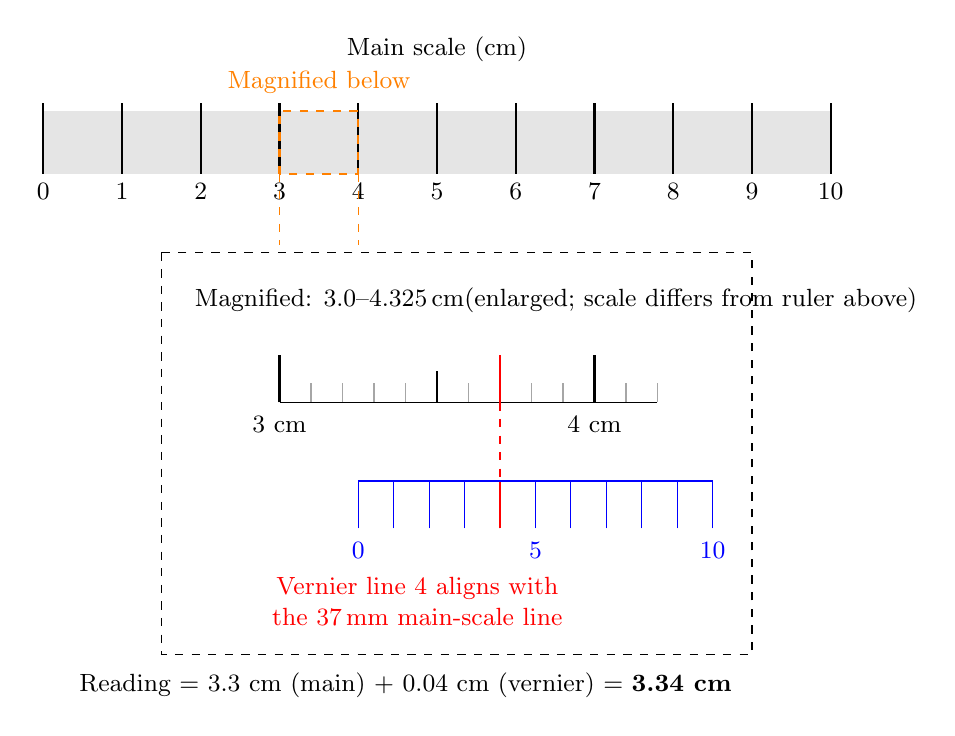
\begin{tikzpicture}[font=\small]

% ===== Overview: full main scale, 0-10 cm =====
\fill[gray!20] (0,-0.4) rectangle (10,0.4);
\foreach \x in {0,1,...,10}
  \draw[black, thick] (\x,-0.4) -- (\x,0.5);
\foreach \x in {0,1,...,10}
  \node[below] at (\x,-0.4) {\x};
\node[above] at (5,0.9) {Main scale (cm)};

% Zoom-region highlight (3 cm to 4 cm) and connector lines to the inset
\draw[orange, dashed, thick] (3,-0.4) rectangle (4,0.4);
\node[above, orange, font=\small] at (3.5,0.5) {Magnified below};
\draw[orange, dashed] (3,-0.4) -- (3,-1.3);
\draw[orange, dashed] (4,-0.4) -- (4,-1.3);

% ===== Magnified inset: 3.0-4.325 cm region, correctly proportioned =====
\begin{scope}[shift={(3,-3.3)}]
  \draw[dashed] (-1.5,1.9) rectangle (6.0,-3.2);
  \node[right, font=\small] at (-1.2,1.30)
    {Magnified: 3.0--4.325\,cm \\(enlarged; scale differs from ruler above)};

  % ----- Main scale, millimetre ticks -----
  % Major (whole cm)
  \draw[thick] (0,0) -- (0,0.6);     \node[below] at (0,-0.05) {3 cm};
  \draw[thick] (4.0,0) -- (4.0,0.6); \node[below] at (4.0,-0.05) {4 cm};
  % Half-cm tick
  \draw (2.0,0) -- (2.0,0.4);
  % Minor mm ticks
  \foreach \x in {0.4,0.8,1.2,1.6,2.4,2.8,3.2,3.6,4.4,4.8}
    \draw[gray!70] (\x,0) -- (\x,0.25);
  % Highlighted coincidence tick: the 37 mm main-scale line
  \draw[red, thick] (2.8,0) -- (2.8,0.6);
  \draw (0,0) -- (4.8,0);

  % ----- Vernier scale: zero at 33.4 mm, 10 divisions = 9 mm total -----
  \foreach \x in {1.0,1.45,1.9,2.35,2.8,3.25,3.7,4.15,4.6,5.05,5.5}
    \draw[blue] (\x,-1.6) -- (\x,-1.0);
  % Coincident vernier line (division 4)
  \draw[red, thick] (2.8,-1.6) -- (2.8,-1.0);
  \node[below, blue] at (1.0,-1.65) {0};
  \node[below, blue] at (3.25,-1.65) {5};
  \node[below, blue] at (5.5,-1.65) {10};
  \draw[blue] (1.0,-1.0) -- (5.5,-1.0);

  % Coincidence guide line
  \draw[red, dashed] (2.8,0) -- (2.8,-1.6);
  \node[below, red, font=\small, align=center] at (1.75,-2.1)
    {Vernier line 4 aligns with\\ the 37\,mm main-scale line};

  % Reading
  \node[align=center] at (1.6,-3.6)
    {Reading = 3.3 cm (main) + 0.04 cm (vernier) = \textbf{3.34 cm}};
\end{scope}

\end{tikzpicture}%
}
\end{center}
\end{diagbox}

\begin{definitionbox}[Scalar Quantity]
A \textbf{scalar quantity} is a physical quantity that is
completely described by its \textbf{magnitude} (size) alone,
together with its unit. Scalars have no direction.

Examples: mass, time, temperature, energy, speed, distance,
pressure, density, electric charge, work.
\end{definitionbox}

\begin{definitionbox}[Vector Quantity]
A \textbf{vector quantity} is a physical quantity that
requires both \textbf{magnitude} and \textbf{direction} to
be completely described.

Examples: displacement, velocity, acceleration, force,
weight, momentum, electric field, magnetic field.
\end{definitionbox}

\begin{misconceptionbox}
Speed and velocity are not the same thing. Speed is a scalar
--- it tells you how fast an object moves. Velocity is a
vector --- it tells you how fast and in which direction.
A car driving at 60 km\,h$^{-1}$ north and another driving
at 60 km\,h$^{-1}$ south have the same speed but opposite
velocities. Similarly, distance and displacement are
different: distance is scalar (total path length),
displacement is vector (straight-line distance from start
to finish, with direction).
\end{misconceptionbox}

Scalars obey ordinary algebra. Vectors obey the laws of
vector addition, which we will explore fully in Chapter 2.
The key point here is that when adding vectors, direction
matters absolutely. Two forces of 5 N each can produce a
resultant force anywhere from 0 N (opposing directions)
to 10 N (same direction), depending on the angle between
them. Two scalar quantities of 5 added together always
give 10.

\begin{realworldbox}[Vectors on Lagos Roads]
Suppose you drive from Ikeja to Victoria Island: first
10 km south along Lagos-Ibadan Expressway, then 8 km
southeast to the Island. Your total distance travelled
is $10 + 8 = 18\ \text{km}$ (scalar addition). But your
displacement --- the straight-line distance from Ikeja
to your final position --- is approximately 15 km at a
bearing of about \SI{155}{\degree} (vector addition). The map cares
about displacement; the fuel gauge cares about distance.
\end{realworldbox}

\vspace{3.4cm}

% ============================================================
\section{Chapter Summary}
% ============================================================

\begin{summarybox}

\textbf{Physical quantities} consist of a numerical value
and a unit. Every equation in Physics must be dimensionally
homogeneous.

\vspace{0.4cm}

\textbf{The seven SI fundamental quantities:}
Length (m), Mass (kg), Time (s), Current (A),
Temperature (K), Amount of substance (mol),
Luminous intensity (cd).

\vspace{0.4cm}

\textbf{Metric prefixes} allow large and small quantities
to be expressed compactly:
$\text{nano}\ (10^{-9})$,
$\text{micro}\ (10^{-6})$,
$\text{milli}\ (10^{-3})$,
$\text{kilo}\ (10^3)$,
$\text{mega}\ (10^6)$,
$\text{giga}\ (10^9)$.

\vspace{0.4cm}

\textbf{Standard form:} $A \times 10^n$, where
$1 \leq A < 10$.

\vspace{0.4cm}

\textbf{Dimensional analysis} checks equations for
consistency and can be used to derive relationships.
Dimensions of fundamental quantities: $[M]$, $[L]$, $[T]$,
$[I]$, $[\Theta]$.

\vspace{0.4cm}

\textbf{Significant figures:}
\begin{itemize}[noitemsep]
  \item Multiplication/division: result takes s.f. of
  least precise measurement
  \item Addition/subtraction: result takes decimal places
  of least precise measurement
\end{itemize}

\vspace{0.4cm}

\textbf{Errors:}
Systematic errors are consistent biases;
random errors are unpredictable fluctuations.
Percentage uncertainty $= (\Delta x / x) \times 100\%$.

\vspace{0.4cm}

\textbf{Scalars} have magnitude only.
\textbf{Vectors} have both magnitude and direction.

\end{summarybox}

% ============================================================
% EXERCISES
% ============================================================
\newpage

\begin{exercisebox}[1]

\subsection*{Section A: Multiple Choice}

\textit{Choose the single most correct answer for each
question. Each question carries 1 mark.}

\vspace{0.3cm}

\textbf{A1.} Which of the following is a fundamental quantity in
the SI system?

\mcoption{A}{Force}
\mcoption{B}{Velocity}
\mcoption{C}{Electric current}
\mcoption{D}{Energy}
\ansref{Ch1-A1}

\vspace{0.4cm}

\textbf{A2.} A length of $3.5 \times 10^{-4}\ \text{m}$
is equivalent to:

\mcoption{A}{$0.035\ \text{mm}$}
\mcoption{B}{$0.35\ \text{mm}$}
\mcoption{C}{$3.5\ \text{mm}$}
\mcoption{D}{$35\ \text{mm}$}
\ansref{Ch1-A2}

\vspace{0.4cm}

\textbf{A3.} The dimension of pressure is:

\mcoption{A}{$[M\,L^{-1}\,T^{-2}]$}
\mcoption{B}{$[M\,L\,T^{-2}]$}
\mcoption{C}{$[M\,L^2\,T^{-2}]$}
\mcoption{D}{$[M\,L^{-2}\,T^{-1}]$}
\ansref{Ch1-A3}

\vspace{0.4cm}

\textbf{A4.} How many significant figures are in the
measurement $0.004\,070\ \text{kg}$?

\mcoption{A}{3}
\mcoption{B}{4}
\mcoption{C}{5}
\mcoption{D}{7}
\ansref{Ch1-A4}

\vspace{0.4cm}

\textbf{A5.} A speed of $108\ \text{km\,h}^{-1}$ is
equal to:

\mcoption{A}{$20\ \text{m\,s}^{-1}$}
\mcoption{B}{$30\ \text{m\,s}^{-1}$}
\mcoption{C}{$40\ \text{m\,s}^{-1}$}
\mcoption{D}{$60\ \text{m\,s}^{-1}$}
\ansref{Ch1-A5}

\vspace{0.4cm}

\textbf{A6.} Which of the following is a vector quantity?

\mcoption{A}{Temperature}
\mcoption{B}{Power}
\mcoption{C}{Momentum}
\mcoption{D}{Mass}
\ansref{Ch1-A6}

\vspace{0.4cm}

\textbf{A7.} The equation $E = mgh$ (where $E$ is energy,
$m$ is mass, $g$ is gravitational field strength, and $h$
is height) is checked by dimensional analysis.
The dimensions of the right-hand side are:

\mcoption{A}{$[M\,L\,T^{-1}]$}
\mcoption{B}{$[M\,L^2\,T^{-2}]$}
\mcoption{C}{$[M\,L^2\,T^{-1}]$}
\mcoption{D}{$[M\,L\,T^{-2}]$}
\ansref{Ch1-A7}

\vspace{0.4cm}

\textbf{A8.} A student measures a rod five times and
obtains the values: 24.3, 24.3, 24.4, 24.3, 24.3 cm.
These results are best described as:

\mcoption{A}{Accurate but not precise}
\mcoption{B}{Precise but not necessarily accurate}
\mcoption{C}{Neither accurate nor precise}
\mcoption{D}{Both accurate and precise}
\ansref{Ch1-A8}

\vspace{0.4cm}

\textbf{A9.} The density of a liquid is
$0.85\ \text{g\,cm}^{-3}$. In SI base units this is:

\mcoption{A}{$8.5\ \text{kg\,m}^{-3}$}
\mcoption{B}{$85\ \text{kg\,m}^{-3}$}
\mcoption{C}{$850\ \text{kg\,m}^{-3}$}
\mcoption{D}{$8500\ \text{kg\,m}^{-3}$}
\ansref{Ch1-A9}

\vspace{0.4cm}

\textbf{A10.} Which of the following equations is
dimensionally inconsistent? (All symbols have their
standard meanings: $v$ = speed, $a$ = acceleration,
$t$ = time, $s$ = displacement, $m$ = mass,
$F$ = force, $E$ = energy)

\mcoption{A}{$v = at$}
\mcoption{B}{$s = \frac{1}{2}at^2$}
\mcoption{C}{$E = mva$}
\mcoption{D}{$F = \frac{E}{s}$}
\ansref{Ch1-A10}

\vspace{0.6cm}

\subsection*{Section B: Theory and Calculations}

\textit{Answer all five questions. Show full working
where calculations are required.}

\vspace{0.3cm}

\textbf{B1.} (a) State the difference between a base
quantity and a derived quantity, giving two examples
of each.\\
(b) The speed of light in a vacuum is
$3.00 \times 10^8\ \text{m\,s}^{-1}$. The distance
from the Sun to the Earth is
$1.50 \times 10^{11}\ \text{m}$.
Calculate the time it takes light to travel from the
Sun to the Earth. Express your answer in minutes and
seconds.
\hfill\ansref{Ch1-B1}

\vspace{0.4cm}

\textbf{B2.} A physical quantity $Q$ is defined by the
equation:
\[
  Q = \frac{F\,\ell^2}{m\,v}
\]
where $F$ is force, $\ell$ is length, $m$ is mass, and
$v$ is speed.

\smallskip

(a) Determine the dimensions of $Q$.

(b) What are the SI units of $Q$?
(c) Is $Q$ a scalar or a vector quantity? Justify your
answer.
\hfill\ansref{Ch1-B2}

\vspace{0.4cm}

\textbf{B3.} A cylindrical steel rod is measured with
a micrometer screw gauge. The diameter is
$d = 4.20 \pm 0.02\ \text{mm}$ and the length is
$L = 85.0 \pm 0.5\ \text{mm}$.

\smallskip

(a) Calculate the volume of the rod using
$V = \frac{\pi d^2 L}{4}$.

(b) Calculate the percentage uncertainty in the volume.
(c) Express the volume with its absolute uncertainty.

($\pi = 3.142$)
\hfill\ansref{Ch1-B3}

\vspace{0.4cm}

\textbf{B4.} The gravitational force $F$ between two
objects depends on their masses $m_1$ and $m_2$, the
distance $r$ between them, and the gravitational
constant $G$.

A student proposes the equation:
\[
  F = \frac{G m_1 m_2}{r^2}
\]
(a) Use dimensional analysis to find the dimensions of
$G$ and hence its SI units.

(b) The gravitational constant is measured to be
$G = 6.674 \times 10^{-11}\ \text{N\,m}^2\text{kg}^{-2}$.
Calculate the gravitational force between a 65 kg person
standing on the surface of the Earth, given that the mass
of the Earth is $5.97 \times 10^{24}\ \text{kg}$ and its
radius is $6.37 \times 10^6\ \text{m}$.

(c) What is the name usually given to this force?
\hfill\ansref{Ch1-B4}

\vspace{0.4cm}

\textbf{B5.} (a) Estimate the total length of blood
vessels in a human body.
Start from the following estimates: the human body
contains approximately $5 \times 10^9$ red blood cells;
each red blood cell passes through a capillary
approximately every 60 seconds; the average speed of
blood in a capillary is approximately
$0.5\ \text{mm\,s}^{-1}$; a capillary is approximately
$1\ \text{mm}$ long.

\smallskip

(b) Express your answer in kilometres.

\smallskip

(c) Compare this length to the circumference of the Earth
($\approx 40\,000\ \text{km}$). How many times could
the blood vessels wrap around the Earth?
\hfill\ansref{Ch1-B5}

\end{exercisebox}

\vspace{0.5cm}

% ============================================================
% ANSWER KEY FOR THIS CHAPTER (goes into answers.tex)
% ============================================================
% Ch1-A1: C (Electric current is one of the seven SI base
%         quantities. Force and energy are derived; velocity
%         is derived from length and time.)
%
% Ch1-A2: B (3.5e-4 m = 3.5e-4 * 1000 mm = 0.35 mm)
%
% Ch1-A3: A (P = F/A = [MLT-2]/[L2] = [ML-1T-2])
%
% Ch1-A4: B (4 s.f.: 4, 0, 7, 0 - the leading zeros are
%         not significant; the trailing zero after 7 is
%         significant because it comes after the decimal.)
%
% Ch1-A5: B (108 / 3.6 = 30 m/s)
%
% Ch1-A6: C (Momentum = mass x velocity, inherits direction
%         from velocity. Temperature, power and mass are
%         all scalars.)
%
% Ch1-A7: B ([M][LT-2][L] = [ML2T-2] = dimension of energy)
%
% Ch1-A8: B (The measurements are consistent with each
%         other - precise. Whether they are accurate
%         depends on the true length, which we are not told.)
%
% Ch1-A9: C (0.85 g/cm3 * 1000 = 850 kg/m3)
%
% Ch1-A10: C (E = mva: [M][LT-1][LT-2] = [ML2T-3] = power,
%          not energy [ML2T-2]. Dimensionally inconsistent.)
% ============================================================